\documentclass[preview]{standalone}
\usepackage{circuitikz}
\usetikzlibrary{shapes.geometric}
\begin{document}
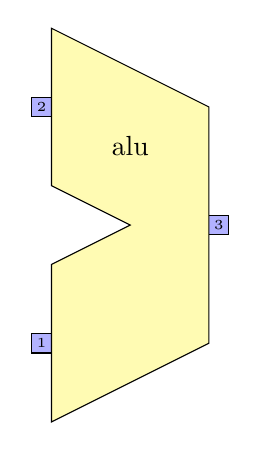
\begin{tikzpicture}
\begin{scope}[shift={(0.000000,0.000000)}]
\begin{scope}[shift={(-0.250000,0.875000)}]\draw [fill=blue!30] (0.000000,0.000000) -- (0.250000,0.000000) -- (0.250000,0.250000) -- (0.000000,0.250000) -- cycle;
\node at (0.125,0.125) {\tiny{1}};
\end{scope}
\begin{scope}[shift={(-0.250000,3.875000)}]\draw [fill=blue!30] (0.000000,0.000000) -- (0.250000,0.000000) -- (0.250000,0.250000) -- (0.000000,0.250000) -- cycle;
\node at (0.125,0.125) {\tiny{2}};
\end{scope}
\begin{scope}[shift={(2.000000,2.375000)}]\draw [fill=blue!30] (0.000000,0.000000) -- (0.250000,0.000000) -- (0.250000,0.250000) -- (0.000000,0.250000) -- cycle;
\node at (0.125,0.125) {\tiny{3}};
\end{scope}
\begin{scope}[shift={(0.875000,0.750000)}]\draw [fill=blue!30] (0.000000,0.000000) -- (0.250000,0.000000) -- (0.250000,0.500000) -- (0.000000,0.500000) -- cycle;
\node at (0.125,0.000000) {\tiny{3}};
\end{scope}
\begin{scope}[shift={(0.875000,0.750000)}]\draw [fill=blue!30] (0.000000,0.000000) -- (0.250000,0.000000) -- (0.250000,0.500000) -- (0.000000,0.500000) -- cycle;
\node at (0.125,0.000000) {\tiny{4}};
\end{scope}
\draw [fill=yellow!30] (0.000000,0.000000) -- (2.000000,1.000000) -- (2.000000,4.000000) -- (0.000000,5.000000) -- (0.000000,3.000000) -- (1.000000,2.500000) -- (0.000000,2.000000) -- cycle;
\node at (1.000000,3.500000) {alu};
\end{scope}
\end{tikzpicture}
\end{document}
